% ***********************************************************
% ******************* PHYSICS HEADER ************************
% ***********************************************************
% Version 2
\documentclass[11pt]{article} 
\usepackage{amsmath} % AMS Math Package
\usepackage{amsthm} % Theorem Formatting
\usepackage{amssymb}	% Math symbols such as \mathbb
\usepackage{graphicx} % Allows for eps images
\usepackage{multicol} % Allows for multiple columns
\usepackage[dvips,letterpaper,margin=0.75in,bottom=0.5in]{geometry}
 % Sets margins and page size
\pagestyle{empty} % Removes page numbers
\makeatletter % Need for anything that contains an @ command 
\renewcommand{\maketitle} % Redefine maketitle to conserve space
{ \begingroup \vskip 10pt \begin{center} \large {\bf \@title}
	\vskip 10pt \large \@author \hskip 20pt \@date \end{center}
  \vskip 10pt \endgroup \setcounter{footnote}{0} }
\makeatother % End of region containing @ commands
\renewcommand{\labelenumi}{(\alph{enumi})} % Use letters for enumerate
% \DeclareMathOperator{\Sample}{Sample}
\let\vaccent=\v % rename builtin command \v{} to \vaccent{}
\renewcommand{\v}[1]{\ensuremath{\mathbf{#1}}} % for vectors
\newcommand{\gv}[1]{\ensuremath{\mbox{\boldmath$ #1 $}}} 
% for vectors of Greek letters
\newcommand{\uv}[1]{\ensuremath{\mathbf{\hat{#1}}}} % for unit vector
\newcommand{\abs}[1]{\left| #1 \right|} % for absolute value
\newcommand{\avg}[1]{\left< #1 \right>} % for average
\let\underdot=\d % rename builtin command \d{} to \underdot{}
\renewcommand{\d}[2]{\frac{d #1}{d #2}} % for derivatives
\newcommand{\dd}[2]{\frac{d^2 #1}{d #2^2}} % for double derivatives
\newcommand{\pd}[2]{\frac{\partial #1}{\partial #2}} 
% for partial derivatives
\newcommand{\pdd}[2]{\frac{\partial^2 #1}{\partial #2^2}} 
% for double partial derivatives
\newcommand{\pdc}[3]{\left( \frac{\partial #1}{\partial #2}
 \right)_{#3}} % for thermodynamic partial derivatives
\newcommand{\ket}[1]{\left| #1 \right>} % for Dirac bras
\newcommand{\bra}[1]{\left< #1 \right|} % for Dirac kets
\newcommand{\braket}[2]{\left< #1 \vphantom{#2} \right|
 \left. #2 \vphantom{#1} \right>} % for Dirac brackets
\newcommand{\matrixel}[3]{\left< #1 \vphantom{#2#3} \right|
 #2 \left| #3 \vphantom{#1#2} \right>} % for Dirac matrix elements
\newcommand{\grad}[1]{\gv{\nabla} #1} % for gradient
\let\divsymb=\div % rename builtin command \div to \divsymb
\renewcommand{\div}[1]{\gv{\nabla} \cdot #1} % for divergence
\newcommand{\curl}[1]{\gv{\nabla} \times #1} % for curl
\let\baraccent=\= % rename builtin command \= to \baraccent
\renewcommand{\=}[1]{\stackrel{#1}{=}} % for putting numbers above =
\newtheorem{prop}{Proposition}
\newtheorem{thm}{Theorem}[section]
\newtheorem{lem}[thm]{Lemma}
\theoremstyle{definition}
\newtheorem{dfn}{Definition}
\theoremstyle{remark}
\newtheorem*{rmk}{Remark}

% ***********************************************************
% ********************** END HEADER *************************
% ***********************************************************
\usepackage{cancel}
\usepackage{verbatim}
\usepackage{graphicx}
\usepackage{enumerate}
\usepackage{appendix}
\title{Comp 251: Assignment 4}
\author{Ian Benlolo 260744397\\McGill University \\}
\begin{document}
\maketitle
\begin{enumerate}[1.]
\item 
\textbf{First Case:} $d<\alpha$: \\
The base case, $T(1)=\Theta(1^{\alpha})=\Theta(1)$ is true because $T(1)=c$.\\
IH: Assume $T(n)=\Theta(n^{\alpha})$. So the induction step follows:\\
$T(bn)= aT(n)+c(bn)^d=\Theta(a(n)^{\alpha})+\Theta((bn)^{d})=\Theta(a(n)^{\alpha})$ since $\alpha > d$.\\
Hence by induction, if $d<\alpha, T(n)=\Theta(n^{\alpha})$.\\

\textbf{Second Case} $d=\alpha$:\\
Base case: $T(i)=\Theta(i^{\alpha}\log(1))=\Theta(1\times0)$ which is true as above.\\
IH: assume $T(n)=\Theta(n^{\alpha}\log(n))$, the induction step follows:\\
$T(bn)=aT(n)+c(bn)^d=\Theta(a(n)^{\alpha}\log(bn))+\Theta((bn)^d)=\Theta(an^{\alpha}\log(bn))+\Theta(a(n)^{\alpha})$ since $\alpha=d \rightarrow T(bn)=\Theta(an^{\alpha}\log(bn))$\\

\textbf{Third case: }$ d>\alpha$:\\
Base case: $T(i)=\Theta(1^d)=\Theta(1)$, same as above.\\
IH: Assume $T(n)=\Theta(n^d)$ then $T(bn)=\Theta((bn)^d)=\Theta(an^d)$.\\
It goes as follows:\\
$T(bn)=aT(n)+c(bn)^d=\Theta(an^d)+\Theta((bn)^d)=\Theta(an^d)$ since $\alpha<d \rightarrow T(bn)=\Theta(an^d)$.\\
Then by induction, if $d>\alpha, T(n)=\Theta(n^d)$.


%% question 2 %%
\item 
	\begin{enumerate}[(a)]
	\item
	To solve this in $O(n^2)$ we would use a nested loop. The first one from $i=0$ to the length of the array and the nested on from $j=i+1$  also to the length of the array. We would keep a variable $max$ within the nested loop we would  check if $a_j-a_i>max$, then you would update $max$ and store the values of $i$ and $j$ at these points. \\
	
	\item
	We start by determining the base case which is if we have one day, we buy and sell on that day which gives no profit. If it isn't so, we split the array into half and the correct indices to buy/sell are in one of the following  three cases:
	\begin{enumerate}[I]
	\item Both in the first half.
	\item Both in the second half.
	\item Each in one of the halves.
	\end{enumerate}
	I and II are trivial; they can be found by simply recursively calling our algorithm. III can be solved by a simple scan over the array and finding these two values. Our recurrence relation is therefore:$T(1)\leq O(1)$ and $T(n) \leq 2T(n / 2) + O(n)$ which is $O(n*\log n)$ time (using the Master Theorem). 
	

	\end{enumerate}
	
\item There are a total of $39$ characters in this sentence. The frequency of each character goes as follows:\\
$$f_t=\frac{6}{39}, f_h=\frac{3}{39}, f_a=\frac{2}{39}, f_{space}=\frac{6}{39}, f_r=\frac{4}{39}, f_u=\frac{1}{39}, f_g=\frac{2}{39}, f_e=\frac{5}{39}, f_l=\frac{2}{39}, $$$$f_y=\frac{1}{39},f_i=\frac{1}{39}, f_d=\frac{1}{39}, f_o=\frac{3}{39}, f_m=\frac{1}{39}, f_.=\frac{1}{39}$$\\Building a binary tree from this using Huffman code, we take the lest frequent nodes, make them siblings, and add their frequencies. Doing this we build the following tree:

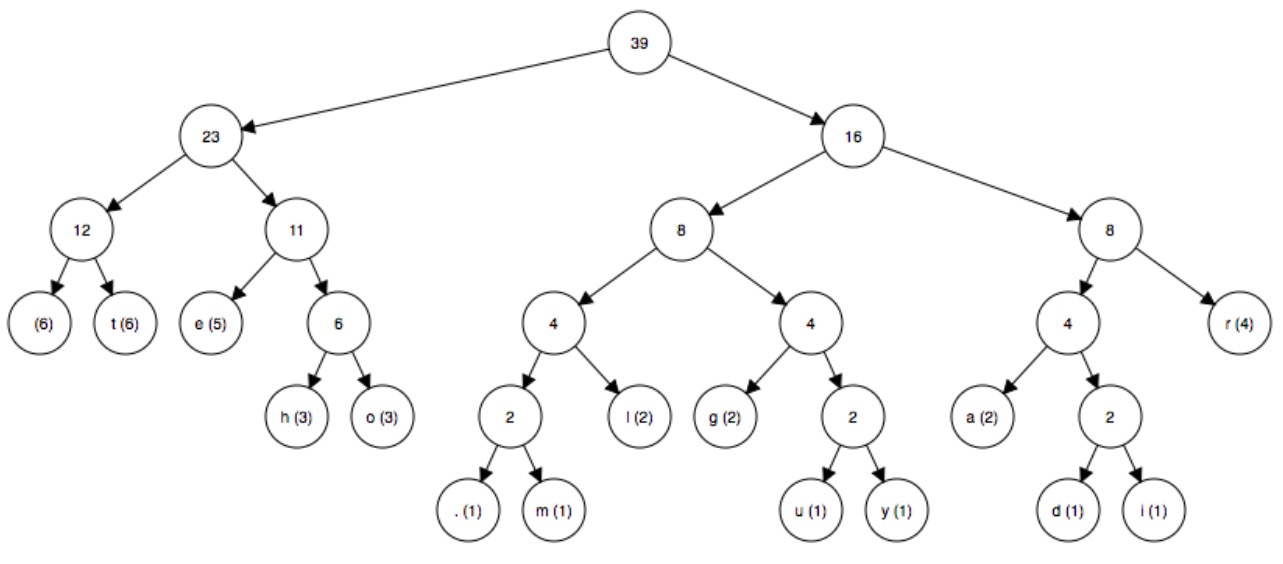
\includegraphics[width=\textwidth]{Huff}

Setting every left-going edge to a $0$ and right-going edge to a $1$ and encoding every letter we get the following:
$$t= 001,\ h=0110,\ a=1100,\ space=000,\ r=111,\ u=10110,\ g=1010,\ e=010,$$$$ l=1001,\ y=10111,\ i=11011,\ d=11010,\ o=0111,\ m=10001,\ .=10000$$
The sentence therefore translates to: \\
$001011011000010001111011010100001110101100100110011011100000111011010110100\\ 0000101100111000111011101111000100000101111010010001011001011110000$\\

%% quesition 4 %%
\item
If we had an input file with, say, n-chars, we'd have $(2^8)^n$ possible inputs. \\
Now suppose you could compress this for all inputs to i chars, with $i<n$, we would be able to form $2^{8i}$ compressions whereas $2^{8i}$ is at most $2^{8n}-1$ possibilities.\\
By the PigeonHole Principle, with $2^{8n}$ items, and $2^{8i}$ containers, there would be at least one container with two items; two chars will have the same compressed string since $2^{8n}>2^{8i}$.

%%  question 5  %%
\item
Algorithm boardCoverDivideAndConquer
input: integer n, cell p
//n=size of the board, p=the cell thats missing
We start by defining the base case, because we are using a recursive algorithm. If we have a $2\times2$ square with one cell missing we fill it with a tile. \\
We split the board to four $n/2\times n/2$ squares. We set a tile in the center of the board such that it covers one tile in each of the quarters which do not contain the missing cell. We now have four boards, each containing one cell "missing"; either covered or the initial missing cell on the board.\\
We now recursively call this algorithm with input $n/2$ and the cell thats missing on each of the $n/2\times n/2$ boards.\\

The time complexity of this $T(n)=4T(n/2)+C$ which is $\Theta(n^2)$, using the Master Theorem. 

%%question 6 %%
\item
Doing this is actually much simpler than it appears. It is taught in almost any basic linear algebra course that the $(i,j)$ element in the $n^{th}$ power of an adjacency matrix counts the number of paths of length $n$ starting at $i$ and ending at $j$. Since we are looking for paths of length $3$ which start and end at the same node, we would take the $3^{rd}$ power of the adjacency matrix $A$. Now, the $i^{th}$ diagonal element in the $A^3$ matrix counts the number of triangles which contains $i$ as one of the nodes. \\
Therefore we would take cube the adjacency matrix, take the trace and divide it by $3$ because a triangle can have $3$ permutations. The time complexity of this would be the time complexity of matrix multiplication, therefore $\Theta(n^{2.81\dots})$ as seen in class, $O(n)$ for the addition and $O(n^{1.585\dots})$ for the division as seen in class. Now, $$\lim_{n\to \inf}\frac{n^{281\dots}+n^{1.585\dots}+n}{n^3}=0$$ therefore this would in fact be $o(n^3)$.

\end{enumerate}

\end{document}